% !TeX program = pdflatex
% =============================================================================
% Aufgabenblatt: Lorentzkraft Teil 1 -- Magnetische Kraft auf stromdurchflossene
% Leiter
% UZH Praktikum I -- Sara Romer Urban, Kantonsschule im Lee, HS2026
% Klassen: 4fh (15.09.2026) + 4cdeg (18.09.2026) -- gemeinsames Material
%
% Uebungsaufgaben fuer die Vor-/Nachbereitung (kein Simulations-/Excel-Inhalt
% bei diesem Thema, siehe institutionen/UZH-Praktikum-I/CLAUDE.md -- die
% Zuordnung Arbeitsblatt/Aufgabenblatt folgt hier trotzdem dem Muster
% "Aufgaben ohne Experimentbezug wandern ins Aufgabenblatt", analog zu
% Kondensatoren/Magnetfelder):
%   - Aufgabe 1 stammt aus arbeitsblatt6-lorentzkraft-teil1.tex (dort als
%     "Uebung: Magnetische Kraft berechnen" entworfen, unveraendert hierher
%     verschoben, damit das Arbeitsblatt bei den drei Experimenten bleibt).
%   - Aufgabe 2 und 3 stammen aus literatur/ (LEIFIphysik-PDFs, siehe
%     Kommentar direkt ueber jeder Aufgabe fuer Quelle/Abbildung -- Zahlen
%     und Aufgabentext von dort uebernommen, Loesungswege selbst
%     nachvollzogen und vollstaendig ausformuliert). Bewusst NICHT
%     aufgenommen: alles zu den sechs Teil-2-Gruppenpuzzle-Anwendungen
%     (Massenspektrograph, Geschwindigkeitsfilter/Wien-Filter, Zyklotron,
%     Hall-Effekt, MHD-Antrieb, Erdmagnetfeld/Magnetosphaere) sowie das
%     LEIFIphysik-"Richtungsregel-Training" (sechsteilige Bildaufgabe) --
%     dessen Teilaufgaben ueberschneiden sich zu stark mit der bereits im
%     Arbeitsblatt vorhandenen Drei-Finger-Regel-Uebung und waeren ohne
%     zweifelsfrei rekonstruierbare Vektorgeometrie aus der Quelle nur mit
%     Raten loesbar gewesen -- deshalb ausgelassen statt geraten.
%
% Bilder: noch keine eingebunden (Stand dieser Fassung) -- Loris ergaenzt sie
% in Bilder/, siehe Bildquellen-Kommentar ueber Aufgabe 2 und 3.
% =============================================================================
\documentclass[addpoints,11pt,a4paper]{exam}

\usepackage[T1]{fontenc}
\usepackage[utf8]{inputenc}
\usepackage[ngerman]{babel}
\usepackage{lmodern}
\usepackage[a4paper,margin=2.2cm,headheight=14pt]{geometry}
\usepackage{amsmath}
\usepackage{amssymb}
\usepackage{siunitx}
% Hausstil: zusammengesetzte Einheiten immer als echter Bruch (\frac), nicht
% als Inline-Schrägstrich oder \tfrac -- gilt global für jedes \si/\SI.
\sisetup{per-mode=fraction,fraction-command=\frac}
\usepackage{array,booktabs,tabularx,multirow}
\usepackage{enumitem}
\usepackage{xcolor}
\usepackage{colortbl}
\usepackage{tikz}
\usepackage{physics}
\usepackage{circuitikz}
\usepackage[most]{tcolorbox}
\usepackage{lastpage}
\usepackage{graphicx}
\usepackage{hyperref}

\usetikzlibrary{arrows.meta,calc,angles,quotes,decorations.markings}

\usepackage{setspace}
\usepackage{needspace}
\setlength{\parindent}{0pt}
\setlength{\parskip}{0.6em}
\setstretch{1.08}
\setlist[itemize]{itemsep=0.4em}

% -----------------------------
% Farben (Corporate-Farbschema Physik KFR)
% -----------------------------
\definecolor{titleblue}{HTML}{183A6B}
\definecolor{accentblue}{HTML}{2E6F9E}
\definecolor{lightblue}{HTML}{EAF4FB}
\definecolor{verylightblue}{HTML}{F7FBFE}
\definecolor{lightgray}{HTML}{F4F6F8}
\definecolor{darkgray}{HTML}{4A4A4A}
\definecolor{accentorange}{HTML}{D9720C}
\definecolor{accentpurple}{HTML}{7B2D8E}
\definecolor{lightorange}{HTML}{FCEEE0}
\definecolor{lightpurple}{HTML}{F3EAF7}

% Links (hyperref): farblich ans Corporate-Farbschema angeglichen.
\hypersetup{
  colorlinks=true,
  urlcolor=accentblue,
  linkcolor=accentblue,
  pdftitle={Aufgabenblatt 5: Lorentzkraft (Teil 1)},
  pdfauthor={Loris Keller}
}

% -----------------------------
% Spaltentypen
% -----------------------------
\newcolumntype{Y}{>{\centering\arraybackslash}X}
\newcolumntype{P}[1]{>{\raggedright\arraybackslash}p{#1}}

% -----------------------------
% Boxen
% -----------------------------
\tcbset{before skip=10pt, after skip=10pt}
\newtcolorbox{titlebox}{
  enhanced,
  colback=titleblue,
  colframe=titleblue,
  boxrule=0pt,
  arc=3mm,
  left=3mm,right=3mm,top=3mm,bottom=3mm
}

\newlength{\aufgabenindent}
\settowidth{\aufgabenindent}{10.\hskip\labelsep}

% Praktikum I: keine farbigen Rahmen fuer Fliesstext-Boxen (nur Formel-,
% Hinweis- und Antwortbox bleiben Boxen) -- siehe
% institutionen/UZH-Praktikum-I/CLAUDE.md, Abschnitt "Boxen-Layout".
\newtcolorbox{taskbox}[1][]{
  enhanced, breakable,
  colback=white, colframe=white, boxrule=0pt,
  left=0mm,right=0mm,top=0mm,bottom=0mm,
  before skip=10pt, after skip=10pt,
  before upper={%
    \def\tmpboxtitle{#1}%
    \ifx\tmpboxtitle\empty\else\noindent\textbf{#1}\par\smallskip\fi
  }
}

% formelbox: Violett, um die zentralen Formeln dieser Einheit hervorzuheben.
\newtcolorbox{formelbox}[1][Formel]{
  enhanced,
  breakable,
  colback=lightpurple,
  colframe=accentpurple,
  title={#1},
  fonttitle=\bfseries,
  boxrule=0.9pt,
  arc=2mm,
  left=5mm,right=5mm,top=2mm,bottom=2mm
}

% hinweisbox: Orange, für wichtige Klarstellungen/Verwechslungswarnungen.
\newtcolorbox{hinweisbox}[1][Hinweis]{
  enhanced,
  breakable,
  colback=lightorange,
  colframe=accentorange,
  title={#1},
  fonttitle=\bfseries,
  boxrule=0.7pt,
  arc=2mm,
  left=5mm,right=5mm,top=2mm,bottom=2mm
}

\newtcolorbox{answerbox}{
  breakable,
  colback=white,
  colframe=gray!55,
  boxrule=0.5pt,
  arc=1.5mm,
  left=2mm,right=2mm,top=2mm,bottom=2mm
}

% --- Lösungen ein-/ausblenden -----------------------------------------------
\noprintanswers
%\printanswers

\pointformat{}
\renewcommand{\solutiontitle}{\noindent\color{titleblue}\textbf{Lösung:}\enspace}

\pagestyle{headandfoot}
\cfoot{\textcolor{darkgray}{Seite \thepage\ von \pageref{LastPage}}}

\newcommand{\Kopfzeile}[4]{%
  \begin{titlebox}
    {\color{white}\sffamily\bfseries\Large #4}
  \end{titlebox}
  \vspace{0.5em}
  \noindent\textbf{Klasse:}~#1 \hfill \textbf{Datum:}~#2 \hfill \textbf{Thema:}~#3
    \hfill \textbf{Lehrperson:}~Loris Keller
  \vspace{0.8em}
  \lhead{\textcolor{darkgray}{#3}}
  \rhead{\textcolor{darkgray}{#4}}
}

\newlength{\antwortraumlen}
\newcommand{\Antwortraum}[1]{%
  \pgfmathsetlength{\antwortraumlen}{#1*2.5cm}%
  \begin{answerbox}
    \rule{0pt}{\antwortraumlen}%
  \end{answerbox}%
}

% Schwierigkeitsgrad: kurze Einstufung direkt unter dem Aufgabentitel, wie
% auf den LEIFIphysik-Quellseiten ("Schwierigkeitsgrad: leichte Aufgabe").
\newcommand{\Schwierigkeit}[1]{%
  \textit{\color{darkgray}Schwierigkeitsgrad: #1}\par\smallskip
}

% Werte für Kopfzeile zentral setzen
\newcommand{\Klasse}{4fh / 4cdeg (SP4)}
\newcommand{\Datum}{15.09.2026 (4fh) / 18.09.2026 (4cdeg)}
\newcommand{\Thema}{Lorentzkraft (Teil 1)}
\newcommand{\ArbeitsblattTitel}{Aufgabenblatt 5: Lorentzkraft (Teil 1)}

\begin{document}

\Kopfzeile{\Klasse}{\Datum}{\Thema}{\ArbeitsblattTitel}

% =============================================================================
% Formelsammlung
% =============================================================================
\begin{formelbox}[Formelsammlung]
\begin{align*}
  F_{\text{mag}} &= I\cdot l\cdot B\cdot\sin\alpha
    &&\text{magnetische Kraft, allgemein}\\
  F_{\text{mag}} &= I\cdot l\cdot B &&\text{Spezialfall } \alpha=90^\circ\\
  B &= \frac{\mu_0}{2\pi}\cdot\frac{I}{r} &&\text{Feld eines geraden Leiters, Abstand } r
\end{align*}
$\mu_0=4\pi\cdot10^{-7}\,\si{\newton\per\ampere\squared}=1{,}26\cdot10^{-6}\,\si{\newton\per\ampere\squared}$;
$I$ in \si{\ampere}; $l,\,r$ in \si{\meter}; $B$ in \si{\tesla}; $\alpha$ =
Winkel zwischen Leiter und Feldlinien.
\end{formelbox}

% =============================================================================
% Aufgabe 1: Magnetische Kraft berechnen (verschoben aus dem Arbeitsblatt)
% =============================================================================
\begin{questions}
\begin{taskbox}[Aufgabe 1: Magnetische Kraft berechnen]
\Schwierigkeit{leicht}
\question Am selben Hufeisenmagnetaufbau wie bei der Leiterschaukel
befindet sich ein einfaches, $\SI{5}{\centi\meter}$ langes, gerades
Leiterstück senkrecht zu den Feldlinien. Der Magnet liefert
$B=\SI{0.3}{\tesla}$, durch den Leiter fliesst ein Strom von
$I=\SI{2}{\ampere}$.
\begin{center}
  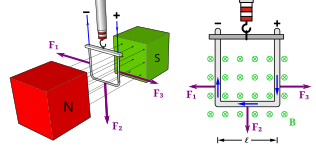
\includegraphics[width=8cm]{Bilder/magnetic-force-measurement-device.pdf}
\end{center}
{\scriptsize So lässt sich die magnetische Kraft auf ein Leiterstück in
der Praxis tatsächlich messen: Ein Federkraftmesser hält den Leiterrahmen,
die Anzeige ändert sich, sobald Strom fliesst.}
\begin{parts}
  \part[2] Berechnen Sie die magnetische Kraft auf das Leiterstück.
  \Antwortraum{2}
  \begin{solution}
  \[
    F = I\cdot l\cdot B = \SI{2}{\ampere}\cdot\SI{0.05}{\meter}\cdot\SI{0.3}{\tesla} = \SI{0.03}{\newton} = \SI{30}{\milli\newton}
  \]
  \end{solution}
  \part[2] Skizzieren Sie $I$, $B$ und $F$ als drei paarweise senkrechte
  Pfeile (analog zur Drei-Finger-Regel) für eine Stromrichtung Ihrer
  Wahl.
  \Antwortraum{2}
  \begin{solution}
  Jede Skizze ist richtig, bei der $I$, $B$ und $F$ paarweise senkrecht
  aufeinander stehen und $F$ tatsächlich der Drei-Finger-Regel (Daumen $I$,
  Zeigefinger $B$, Mittelfinger $F$) für die gewählte Stromrichtung
  entspricht.
  \end{solution}
\end{parts}
\end{taskbox}
\end{questions}

% =============================================================================
% Aufgabe 2: Kraft zwischen den Leitungen einer Gleichspannungs-Freileitung
% Quelle: literatur/Kraft zwischen den Leitungen einer
%   Gleichspannungs-Freileitung _ LEIFIphysik.pdf (Schwierigkeitsgrad dort:
%   leichte Aufgabe). BILD: Abb. 1 dieser Quelle (Foto der FennoSkan-HGÜ-
%   Freileitung, Rauma/Finnland) -- rein motivierend/dekorativ, für die
%   Lösung nicht nötig (alle Werte stehen im Aufgabentext).
% =============================================================================
\begin{questions}
\begin{taskbox}[Aufgabe 2: Kraft zwischen den Leitungen einer Gleichspannungsfreileitung]
\Schwierigkeit{leicht}
\question Eine Hochspannungs-Gleichstrom-Freileitung überträgt eine
Leistung von $P=\SI{600}{\mega\watt}$ bei einer Spannung von
$U=\SI{1150}{\kilo\volt}$. Auf einem $l=\SI{100}{\meter}$ langen
Abschnitt verlaufen zwei ihrer Leitungen im Abstand $r=\SI{0.80}{\meter}$
parallel zueinander, wobei der Strom in den beiden Leitungen in
\textbf{entgegengesetzte} Richtungen fliesst.
\begin{center}
  % BILD: Bilder/hguue-freileitung.jpg (o.ä.) -- siehe Kommentar oben.
\end{center}
\begin{parts}
  \part[1] Berechnen Sie den Strom $I$ in den Leitungen.
  \Antwortraum{1}
  \begin{solution}
  \[
    I = \frac{P}{U} = \frac{\SI{600e6}{\watt}}{\SI{1150e3}{\volt}} \approx \SI{522}{\ampere}
  \]
  \end{solution}
  \part[1] Berechnen Sie die magnetische Flussdichte $B$, die eine der
  beiden Leitungen am Ort der jeweils anderen erzeugt.
  \Antwortraum{1}
  \begin{solution}
  \[
    B = \frac{\mu_0}{2\pi}\cdot\frac{I}{r}
      = \frac{4\pi\cdot10^{-7}\,\si{\newton\per\ampere\squared}}{2\pi}\cdot\frac{\SI{522}{\ampere}}{\SI{0.80}{\meter}}
  \]
  \[
    B = 2\cdot10^{-7}\,\si{\newton\per\ampere\squared}\cdot\frac{\SI{522}{\ampere}}{\SI{0.80}{\meter}}
      \approx \SI{1.3e-4}{\tesla} = \SI{130}{\micro\tesla}
  \]
  \end{solution}
  \part[1] Berechnen Sie die magnetische Kraft auf den betrachteten
  $\SI{100}{\meter}$ langen Leitungsabschnitt.
  \Antwortraum{1}
  \begin{solution}
  Die beiden Leitungen stehen senkrecht zum jeweils anderen Feld
  ($\alpha=90^\circ$), also:
  \[
    F_{\text{mag}} = I\cdot l\cdot B = \SI{522}{\ampere}\cdot\SI{100}{\meter}\cdot\SI{1.3e-4}{\tesla} \approx \SI{6.8}{\newton}
  \]
  \end{solution}
  \part[1] Ziehen sich die beiden Leitungen an oder stossen sie sich ab?
  Begründen Sie mit der Drei-Finger-Regel.
  \Antwortraum{2}
  \begin{solution}
  Bei \textbf{entgegengesetzt} gerichteten Strömen stossen sich zwei
  parallele Leiter ab (vgl. Experiment 2 im Arbeitsblatt). Die beiden
  Leitungen der Freileitung stossen sich also mit $F_{\text{mag}}\approx\SI{6.8}{\newton}$ ab.
  \end{solution}
\end{parts}
\end{taskbox}
\end{questions}

% =============================================================================
% Aufgabe 3: Kraft auf einen Leiterrahmen
% Quelle: literatur/Kraft auf Leiterrahmen _ LEIFIphysik.pdf. BILD: Abb. 1
%   dieser Quelle (Draufsicht, zwei Fälle: Rahmen mit Breite l1 = 10 cm
%   teilweise im Feld, Rahmen mit Breite l2 = 20 cm vollständig im Feld) --
%   für diese Aufgabe hilfreich, da sie die Feldgrenze visuell zeigt, wird
%   im Aufgabentext unten aber vollständig in Worten beschrieben.
% =============================================================================
\begin{questions}
\begin{taskbox}[Aufgabe 3: Kraft auf einen Leiterrahmen]
\Schwierigkeit{mittelschwer}
\question Ein rechteckiger Leiterrahmen trägt einen Strom von
$I=\SI{5.0}{\ampere}$. Er hängt teilweise in einem begrenzten homogenen
Magnetfeld $B=\SI{0.20}{\tesla}$, das senkrecht aus der Zeichenebene
herauszeigt (Draufsicht). Die Feldgrenze verläuft waagrecht; der Rahmen
taucht von oben senkrecht in das Feld ein.
\begin{center}
  % BILD: Bilder/leiterrahmen-im-feld.svg (o.ä.) -- siehe Kommentar oben.
\end{center}
\begin{parts}
  \part[2] In einer ersten Situation taucht der Rahmen so weit ein, dass
  nur seine untere, waagrechte Kante der Breite $l_1=\SI{10}{\centi\meter}$
  vollständig im Feld liegt; die beiden seitlichen (senkrechten) Kanten
  ragen mit gleich langen Stücken ins Feld hinein. Begründen Sie, warum
  sich die Kräfte auf die beiden seitlichen Kanten gegenseitig aufheben,
  und berechnen Sie die resultierende Kraft auf den Rahmen.
  \Antwortraum{2}
  \begin{solution}
  In den beiden seitlichen Kanten fliesst der Strom in \textbf{entgegen\-gesetzte}
  Richtungen (der Rahmen ist geschlossen), aber beide gleich langen
  Teilstücke liegen im selben Feld $B$. Nach der Drei-Finger-Regel zeigen
  die beiden Kräfte deshalb in entgegengesetzte Richtungen und sind
  gleich gross, sie heben sich also auf. Nur die untere Kante trägt
  netto bei:
  \[
    F_{\text{mag}} = I\cdot l_1\cdot B = \SI{5.0}{\ampere}\cdot\SI{0.10}{\meter}\cdot\SI{0.20}{\tesla} = \SI{0.10}{\newton}
  \]
  Die Kraft zieht den Rahmen weiter ins Feld hinein.
  \end{solution}
  \part[2] In einer zweiten Situation ist der Rahmen so weit eingetaucht,
  dass er mit seiner vollen Breite $l_2=\SI{20}{\centi\meter}$ und all
  seinen Kanten vollständig im homogenen Feld liegt. Begründen Sie, wie
  gross die resultierende Kraft auf den Rahmen jetzt ist.
  \Antwortraum{2}
  \begin{solution}
  Jetzt liegen alle vier Kanten vollständig im selben homogenen Feld
  $B$. Für jedes der beiden gegenüberliegenden Kantenpaare (oben/unten
  und links/rechts) fliesst der Strom in entgegengesetzte Richtungen
  durch dasselbe Feld, die Kräfte auf jedes Paar heben sich also
  gegenseitig auf:
  \[
    F_{\text{gesamt}} = 0
  \]
  Ein vollständig in einem homogenen Feld liegender, stromdurchflossener
  Rahmen erfährt keine resultierende Kraft, sondern höchstens ein
  Drehmoment (falls er nicht parallel zum Feld ausgerichtet ist).
  \end{solution}
\end{parts}
\end{taskbox}
\end{questions}

\end{document}
